\section*{Lecture 15}

\subsection*{1.} Consider the mixing problem depicted in \textbf{\autoref{fig:f15_1}} (assuming oil and water is always well-mixed). Derive the system of equations that describes the dynamics of the amount $y_1(t)$ of oil in tank $T_1$, the amount $y_2(t)$ of oil in tank $T_2$ and the amount $y_3(t)$ of oil in tank $T_3$. Here, $t$ denotes time. (You do not need to solve the system of equations.)
\begin{figure} [ht]
  \centering
  \caption{}
  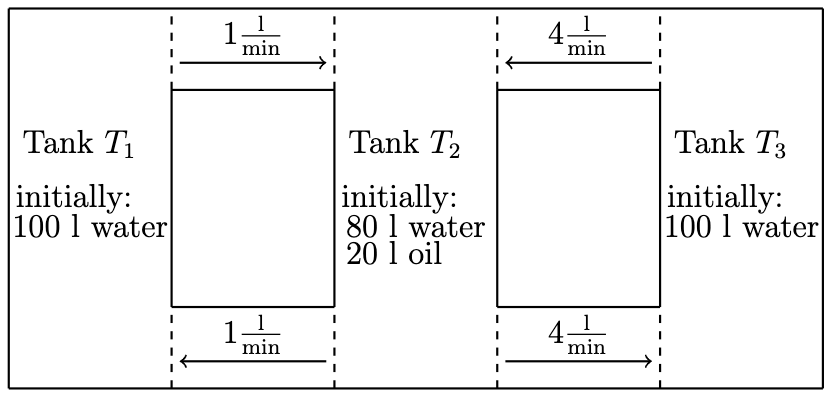
\includegraphics[width=0.5\linewidth]{../figures/f15_1.png}
  \label{fig:f15_1}
\end{figure}
\bigbreak
We will consider the change in the amount of oil in each tank for a small time interval $\Delta t$. For the first tank we have:
\[ 
y_1(t+\Delta t) = y_1(t) + \text{inflow} \cdot \Delta t - \text{outflow} \cdot \Delta t = y_1(t) + \num{0,01} y_2(t) \Delta t - \num{0,01} y_1(t) \Delta t
.\]
We will now subtract by $y_1(t)$ and divide by $\Delta t$ to get
\[ 
\frac{y_1 (t + \Delta t) - y_1(t)}{\Delta t} = \num{0,01} y_2(t) - \num{0,01} y_1(t)
.\]
For $\Delta t \to 0$ we get
\[ 
\lim_{\Delta t \to 0} \frac{y_1 (t + \Delta t) - y_1(t)}{\Delta t} = y_1'(t) = \num{0,01} y_2(t) - \num{0,01} y_1(t)
.\]
Following the same procedure for $T_2$ we get
\[ 
y_2'(t) = \num{0,01} y_1(t) - \num{0,05} y_2(t) + \num{0,04} y_3(t)
.\]
And for $T_3$ we get
\[ 
y_3'(t) = \num{0,04} y_2(t) - \num{0,04} y_3(t)
.\]
This gives the following system of ODEs:
\begin{align*}
  y_1'(t) &= -\num{0,01} y_1(t) + \num{0,01} y_2(t) \\
  y_2'(t) &= \num{0,01} y_1(t) - \num{0,05} y_2(t) + \num{0,04} y_3(t) \\
  y_3'(t) &= \num{0,04} y_2(t) - \num{0,04} y_3(t)
.\end{align*}
If we want to rewrite this on matrix form we can define:
\begin{align*}
  \Vec{y}(t) &= \begin{pmatrix}
  y_1(t)\\
  y_2(t)\\
  y_3(t)\\
  \end{pmatrix} \\
  \Vec{y}'(t) &= \begin{pmatrix}
  y_1'(t)\\
  y_2'(t)\\
  y_3'(t)\\
  \end{pmatrix} \\
    A &= \begin{pmatrix}
    - \num{0,01}  & \num{0,01}  & 0\\
    \num{0,01}  & -\num{0,05}  & \num{0,04} \\
    0 & \num{0,04}  & -\num{0,04} \\
    \end{pmatrix}
.\end{align*}
And write the system as:
\[ 
\Vec{y}'(t) = A \Vec{y}(t)
.\]


\subsection*{2.} Consider the mixing problem depicted in \textbf{\autoref{fig:f15_2}} (assuming oil and water is always well-mixed). Derive the system of equations that describe the dynamics of the amount $y_1(t)$ of oil in tank $T_1$, and the amount $y_2(t)$ of oil in tank $T_2$. Here, $t$ denotes time. (You do not need to solve the system of equations).
\begin{figure} [ht]
  \centering
  \caption{}
  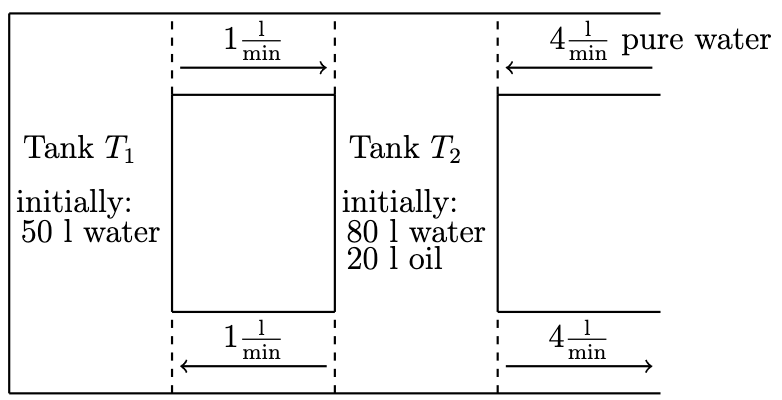
\includegraphics[width=0.5\linewidth]{../figures/f15_2.png}
  \label{fig:f15_2}
\end{figure}
\bigbreak
Here we can follow the same procedure as above and get
\begin{align*}
  y_1'(t) &= -\num{0,02} y_1(t) + \num{0,01} y_2(t) \\
  y_2'(t) &= \num{0,02} y_1(t) - \num{0,05} y_2(t)
.\end{align*}
Which can be rewritten as
\begin{align*}
  A &= \begin{pmatrix}
  -\num{0,02}  & \num{0,01} \\
  \num{0,02}  & -\num{0,05} \\
  \end{pmatrix} \\
    \Vec{y}'(t) &= A\Vec{y}(t)
.\end{align*}


\subsection*{3.} Solve the system of ODEs
\begin{align*}
  y_1'(t) &= y_1(t) + y_2(t) \\
  y_2'(t) &= y_1(t) + y_2(t)
.\end{align*}
\bigbreak
We have the above ODEs which gives:
\begin{align*}
  \Vec{y}'(t) &= \begin{pmatrix}
  y_1'(t)\\
  y_2'(t)\\
  \end{pmatrix} \\
  \Vec{y}(t) &= \begin{pmatrix}
  y_1(t)\\
  y_2(t)\\
  \end{pmatrix} \\
    A &= \begin{pmatrix}
    1 & 1\\
    1 & 1\\
    \end{pmatrix} \\
  \Vec{y}'(t) &= A \Vec{y}(t)
.\end{align*}
Now we must find the eigenvalues of A. To do this we need to solve the characteristic equation:
\[ 
\mathrm{det}(A - \lambda I) = 0
.\]
Which gives
\[ 
\mathrm{det}(A - \lambda I) = \left| \begin{array}{cc}
1 - \lambda & 1\\
1 & 1 - \lambda\\
\end{array} \right| = (1 - \lambda)^2 - 1 = 0
.\]
Which has the solutions $\lambda_1 = 0$ and $\lambda_2 = 2$. Now we must find the eigenvector corresponding to each of the eigenvalues. For $\lambda_1$ we get the condition
\[ 
A \Vec{x}^{(1)} = \lambda_1 \Vec{x}^{(1)} \implies A \Vec{x}^{(1)} = \Vec{0} \implies \begin{pmatrix}
1 & 1\\
1 & 1\\
\end{pmatrix} \begin{pmatrix}
x_1^{(1)}\\
x_2^{(1)}\\
\end{pmatrix} = \Vec{0}
.\]
Here we can quickly see that we can simply choose $\Vec{x}^{(1)} = \begin{pmatrix}
1\\
-1\\
\end{pmatrix}$. For $\lambda_2 = 2$ we get
\[ 
A \Vec{x}^{(2)} = \lambda_2 \Vec{x}^{(2)} \implies (A-2I) \Vec{x}^{(2)} = \Vec{0} \implies \begin{pmatrix}
  -1 & 1\\
  1 & -1\\
\end{pmatrix} \begin{pmatrix}
x_1^{(2)}\\
x_2^{(2)}\\
\end{pmatrix} = \Vec{0}
.\]
Here we can choose $\Vec{x}^{(2)} = \begin{pmatrix}
1\\
1\\
\end{pmatrix}$. Together these two form the basis:
\[ 
\Vec{y}_1(t) = \Vec{x}^{(1)} e^{\lambda_1 t} = \begin{pmatrix}
1\\
-1\\
\end{pmatrix}, \Vec{y}_2(t) = \Vec{x}^{(2)} e^{\lambda_2 t} = \begin{pmatrix}
1\\
1\\
\end{pmatrix} e^{2t}
.\]
The general solution then is:
\[ 
\Vec{y}(t) = c_1 \Vec{y}_1(t) + c_2 \Vec{y}_2(t) = c_1 \begin{pmatrix}
1\\
-1\\
\end{pmatrix} + c_2 \begin{pmatrix}
1\\
1\\
\end{pmatrix} e^{2t}
.\]



\subsection*{4.} Solve the system of ODEs
\begin{align*}
  y'_1(t) &= y_1(t) \\
  y_2'(t) &= 2y_2(t)
.\end{align*}
\bigbreak
This time we have:
\[ 
A = \begin{pmatrix}
1 & 0\\
0 & 2\\
\end{pmatrix}
.\]
To find the eigenvalues of $A$ we follow the same procedure as in Exercise 3. We simply solve the characteristic equation as
\[ 
\mathrm{det}(A - \lambda I) = \left| \begin{array}{cc}
1 - \lambda & 0\\
0 & 2 - \lambda\\
\end{array} \right| = (1-\lambda)(2-\lambda) = 0 \implies \lambda_1 = 1, \lambda_2 = 2
.\]
The eigenvector for $\lambda_1 = 1$ can be found as
\[ 
A \Vec{x}^{(1)} = \lambda_1 \Vec{x}^{(1)} \implies (A-I) \Vec{x}^{(1)} = \Vec{0} \implies \begin{pmatrix}
0 & 0\\
0 & 1\\
\end{pmatrix} \begin{pmatrix}
x_1^{(1)}\\
x_2^{(1)}\\
\end{pmatrix}
.\]
Here we choose $\Vec{x}^{(1)} = \begin{pmatrix}
1\\
0\\
\end{pmatrix}$. For $\lambda_2 = 2$ we have
\[ 
A \Vec{x}^{(2)} = \lambda_2 \Vec{x}^{(2)} \implies (A - 2I) \Vec{x}^{(2)} = \Vec{0} \implies \begin{pmatrix}
  -1 & 0\\
  0 & 0\\
\end{pmatrix} \begin{pmatrix}
x_1^{(2)}\\
x_2^{(2)}\\
\end{pmatrix} = \Vec{0}
.\]
Here we choose $\Vec{x}^{(2)} = \begin{pmatrix}
0\\
1\\
\end{pmatrix}$. This gives the basis:
\[ 
\Vec{y}_1 (t) = \Vec{x}^{(1)} e^{\lambda_1 t} = \begin{pmatrix}
1\\
0\\
\end{pmatrix} e^{t}, \Vec{y}_2(t) = \Vec{x}^{(2)} e^{\lambda_2 t} = \begin{pmatrix}
0\\
1\\
\end{pmatrix} e^{2t}
.\]




\subsection*{5.} Solve the system of ODEs
\begin{align*}
  y_1'(t) &= y_1 (t) \\
  y_2'(t) &= y_2(t) 
.\end{align*}
\textit{Hint:} Linearly independent eigenvectors corresponding to the same eigenvalue may be used for the definition of basis solutions.
\bigbreak
This time we have
\[ 
A = \begin{pmatrix}
1 & 0\\
0 & 1\\
\end{pmatrix}
.\]
To find the eigenvalues of $A$ we simply follow the same procedure as in the previous exercises. We simply solve the characteristic equation as
\[ 
\mathrm{det}(A - \lambda I) = \left| \begin{array}{cc}
1-\lambda & 0\\
0 & 1-\lambda\\
\end{array} \right| = (1-\lambda)^2 = 0 \implies \lambda_1 = 1, \lambda_2 = 1
.\]
The eigenvectors for $\lambda_1 = \lambda_2 = 1$ can be found as
\[ 
A \Vec{x} = \lambda_1 \Vec{x} \implies (A-I) \Vec{x} = \Vec{0} \implies \begin{pmatrix}
0 & 0\\
0 & 0\\
\end{pmatrix} \begin{pmatrix}
x_1\\
x_2\\
\end{pmatrix}= \Vec{0}
.\]
Here both $x_1$ and $x_2$ are arbitrary so we choose linearly independent eigenvectors as:
\[ 
\Vec{x}^{(1)} = \begin{pmatrix}
1\\
0\\
\end{pmatrix}, \Vec{x}^{(2)} = \begin{pmatrix}
0\\
1\\
\end{pmatrix}
.\]
This gives the basis solutions
\[ 
  \Vec{y}_1(t) = \Vec{x}^{(1)} e^{\lambda_1 t} = \begin{pmatrix}
  1\\
  0\\
  \end{pmatrix} e^{t}, \Vec{y}_2(t) = \Vec{x}^{(2)} e^{\lambda_2 t} = \begin{pmatrix}
  0\\
  1\\
  \end{pmatrix} e^{t}
.\]
The general solution therefore becomes
\[ 
\Vec{y}(t) = c_1 \Vec{y}_1(t) + c_2 \Vec{y}_2(t) = c_1 \begin{pmatrix}
1\\
0\\
\end{pmatrix} e^{t} + c_2 \begin{pmatrix}
0\\
1\\
\end{pmatrix} e^{t}
.\]

\subsection*{6.} Solve the system of ODEs
\begin{align*}
  y_1''(t) &= 3y_1(t) + 4y_2(t) \\
  y_2''(t) &= y_1(t) + 3y_2(t)
.\end{align*}
\bigbreak
This time we can define:
\[ 
\Vec{y}(t) = \begin{pmatrix}
y_1(t)\\
y_2(t)\\
\end{pmatrix}, \Vec{y}''(t) = \begin{pmatrix}
y_1''(t)\\
y_2''(t)\\
\end{pmatrix}, A = \begin{pmatrix}
3 & 4\\
1 & 3\\
\end{pmatrix}
.\]
And we therefore want to solve
\[ 
\Vec{y}''(t) = A \Vec{y}(t)
.\]
We assume a solution of the same form as in the previous exercises, that is $\Vec{y}(t) = \Vec{x} e^{\omega t}$. Therefore we get
\[ 
\Vec{y}''(t) = A \Vec{y}(t) \implies \Vec{x} \omega^2 e^{\omega t} = A \Vec{x} e^{\omega t}\implies \omega^2 \Vec{x} = A \Vec{x}
.\]
Therefore we see that $\omega^2 = \lambda$ in the previous sense. Therefore we just need to solve for $\lambda$ in $\mathrm{det}(A-\lambda I ) = 0$ as:
\[ 
\mathrm{det}(A - \lambda I) = \left| \begin{array}{cc}
3-\lambda & 4\\
1 & 3-\lambda\\
\end{array} \right| = (3 - \lambda)^2 - 4 = 0 \implies \lambda_1 = 1, \lambda_2 = 5
.\]
The eigenvector for $\lambda_1 = 1$ can be found as
\[ 
A \Vec{x}^{(1)} = \lambda_1 \Vec{x}^{(1)} \implies (A - I)\Vec{x}^{(1)} = \Vec{0} \implies \begin{pmatrix}
2 & 4\\
1 & 2\\
\end{pmatrix} \begin{pmatrix}
x_1^{(1)}\\
x_2^{(1)}\\
\end{pmatrix} = \Vec{0}
.\]
Here we choose
\[ 
\Vec{x}^{(1)} = \begin{pmatrix}
2\\
-1\\
\end{pmatrix}
.\]
The eigenvector for $\lambda_2 = 5$ can be found as
\[ 
A \Vec{x}^{(2)} = \lambda_2 \Vec{x}^{(2)} \implies (A - 5I) \Vec{x}^{(2)} = \Vec{0} \implies \begin{pmatrix}
-2 & 4\\
1 & -2\\
\end{pmatrix} \begin{pmatrix}
x_1^{(2)}\\
x_2^{(2)}\\
\end{pmatrix} = \Vec{0}
.\]
Here we choose
\[ 
  \Vec{x}^{(2)} = \begin{pmatrix}
  2\\
  1\\
  \end{pmatrix}
.\]
All the possible values for $\omega$ are
\begin{align*}
  \omega^2 &= \lambda_1 \implies \omega_1 = 1, \omega_2 = -1 \\
  \omega^2 &= \lambda_2 \implies \omega_3 = \sqrt{5}, \omega_4 = - \sqrt{5}
.\end{align*}
The basis solutions are all given as
\[ 
\Vec{y}(t) = \Vec{x} e^{\omega t}
.\]
These are all in all
\begin{align*}
  \Vec{y}_1(t) &= \begin{pmatrix}
  2\\
  -1\\
  \end{pmatrix} e^{t} \\
  \Vec{y}_2(t) &= \begin{pmatrix}
  2\\
  -1\\
  \end{pmatrix} e^{-t} \\
  \Vec{y}_3(t) &= \begin{pmatrix}
  2\\
  1\\
  \end{pmatrix} e^{\sqrt{5}t} \\
    \Vec{y}_4(t) &= \begin{pmatrix}
    2\\
    1\\
    \end{pmatrix} e^{-\sqrt{5}t}
.\end{align*}
The general solution is therefore
\[ 
\Vec{y}(t) = c_1 \begin{pmatrix}
2\\
-1\\
\end{pmatrix} e^{t} + c_2 \begin{pmatrix}
2\\
-1\\
\end{pmatrix} e^{-t} + c_3\begin{pmatrix}
2\\
1\\
\end{pmatrix} e^{\sqrt{5}t} + c_4 \begin{pmatrix}
2\\
1\\
\end{pmatrix} e^{-\sqrt{5}t}
.\]



\subsection*{7.} Rewrite
\[ 
y'''(t) + y''(t) + y'(t) + y(t) = 0
\]
as a system of first order ODEs.
\bigbreak
We first define the new functions
\begin{align*}
  y_1(t) &= y(t) \\
  y_2(t) &= y'(t) \\
  y_3(t) &= y''(t)
.\end{align*}
Our system of first order ODEs are therefore
\begin{align*}
  y_1'(t) &= y_2(t) \\
  y_2'(t) &= y_3(t) \\
  y_3'(t) &= - y_3(t) - y_2(t) - y_1(t)
.\end{align*}
And this can be written on the standard form by first defining:
\begin{align*}
  \Vec{y}(t) &= \begin{pmatrix}
  y_1(t)\\
  y_2(t)\\
  y_3(t)\\
  \end{pmatrix} \\
  \Vec{y}'(t) &= \begin{pmatrix}
  y_1'(t)\\
  y_2'(t)\\
  y_3'(t)\\
  \end{pmatrix} \\
    A &= \begin{pmatrix}
    0 & 1 & 0\\
    0 & 0 & 1\\
    -1 & -1 & -1\\
    \end{pmatrix}
.\end{align*}
And writing it all as
\[ 
\Vec{y}'(t) = A\Vec{y}(t)
.\]



\subsection*{8.} Find the general solution of
\[ 
y''(t) - y'(t) = 0
\]
by using theory of systems of first order ODEs.
\bigbreak
We define
\begin{align*}
  y_1(t) &= y(t) \\
  y_2(t) &= y'(t)
.\end{align*}
And our system of first order ODEs therefore becomes
\begin{align*}
  y_1'(t) &= y_2(t) \\
  y_2'(t) &= y_2(t)
.\end{align*}
We can now follow the same procedure as in many of the previous exercises as we have
\[ 
A = \begin{pmatrix}
0 & 1\\
0 & 1\\
\end{pmatrix}
.\]
The eigenvalues of $A$ can be found as
\[ 
\mathrm{det}(A - \lambda I) = \left| \begin{array}{cc}
-\lambda & 1\\
0 & 1 - \lambda\\
\end{array} \right| = -\lambda(1-\lambda) = 0 \implies \lambda_1 = 0, \lambda_2 = 1
.\]
The eigenvector for $\lambda_1 = 0$ can be found as
\[ 
A \Vec{x} = \lambda \Vec{x} \implies A \Vec{x} = \Vec{0} \implies \begin{pmatrix}
0 & 1\\
0 & 1\\
\end{pmatrix} \begin{pmatrix}
x_1^{(1)}\\
x_2^{(1)}\\
\end{pmatrix} = \Vec{0}
.\]
Here we choose
\[ 
\Vec{x}^{(1)} = \begin{pmatrix}
1\\
0\\
\end{pmatrix}
.\]
The eigenvector for $\lambda_2 = 1$ can be found as
\[ 
A \Vec{x} = \lambda \Vec{x} \implies (A - I) \Vec{x} = \Vec{0} \implies \begin{pmatrix}
-1 & 1\\
0 & 0\\
\end{pmatrix} \begin{pmatrix}
x_1^{(1)}\\
x_2^{(1)}\\
\end{pmatrix} = \Vec{0}
.\]
Here we choose
\[ 
\Vec{x}^{(2)} = \begin{pmatrix}
1\\
1\\
\end{pmatrix}
.\]
This gives the basis solutions
\[ 
\Vec{y}_1(t) = \Vec{x}^{(1)} e^{\lambda_1 t} = \begin{pmatrix}
1\\
0\\
\end{pmatrix}, \Vec{y}_2(t) = \Vec{x}^{(2)} e^{\lambda_2 t} = \begin{pmatrix}
1\\
1\\
\end{pmatrix} e^{t}
.\]
And the general solution is therefore
\[ 
\Vec{y}(t) = c_1 \begin{pmatrix}
1\\
0\\
\end{pmatrix} + c_2 \begin{pmatrix}
1\\
1\\
\end{pmatrix} e^{t}
.\]
Since $y(t)$ is the first entry in $\Vec{y}(t)$ as
\[ 
\Vec{y}(t) = \begin{pmatrix}
y_t\\
y_t'\\
\end{pmatrix}
.\]
The solution to the original ODE is
\[ 
y(t) = c_1 + c_2 e^{t}
.\]

